% Include from the sabmod repository root, with graphicx loaded.
% Default: show provenance. Call \showscriptprovenancefalse to hide it.
\newif\ifshowscriptprovenance
\showscriptprovenancetrue
\providecommand{\scriptprovenance}[1]{%
  \ifshowscriptprovenance\space Scripts: \texttt{\detokenize{#1}}.\fi}

\begin{figure}[htbp]
  \centering
  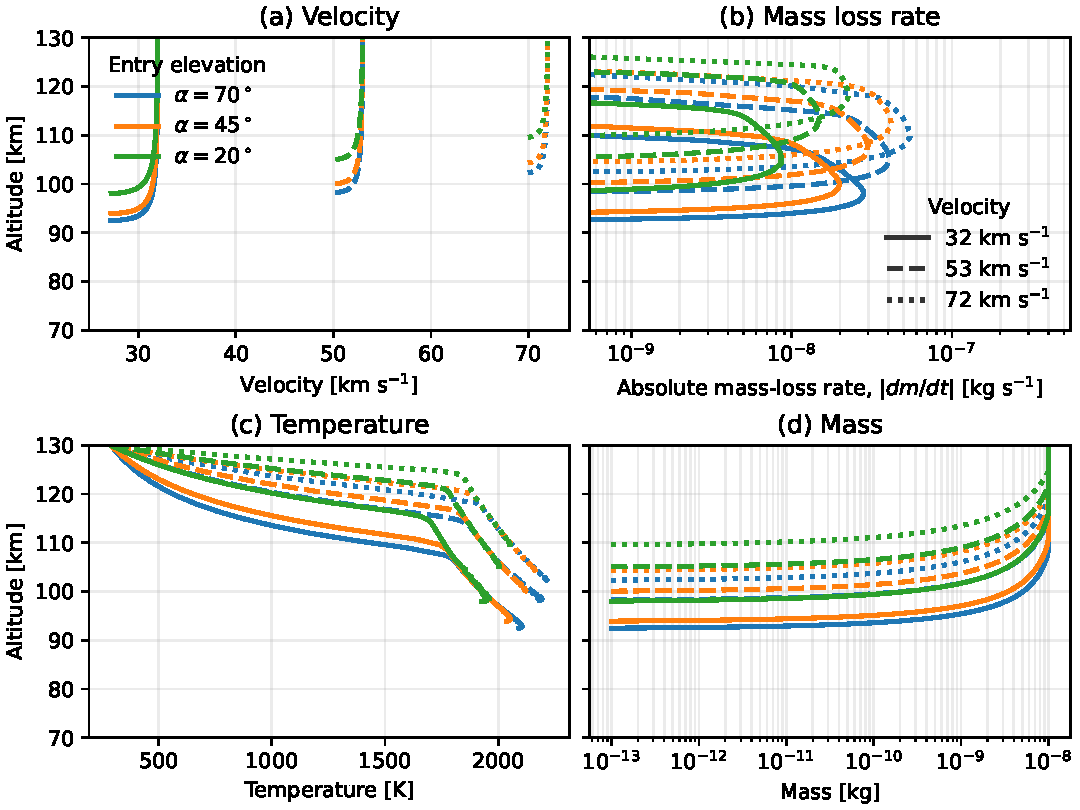
\includegraphics[width=\linewidth]{reproduction/figures/meteor_ablation_single_column.pdf}
  \caption{Reproduced velocity, absolute mass-loss rate, temperature, and
  remaining mass for cometary meteoroids with initial mass $10^{-8}$~kg.
  Entry elevation angles above the horizon are $70^\circ$, $45^\circ$, and
  $20^\circ$; entry speeds are 32, 53, and 72~km~s$^{-1}$.
  The atmosphere is MSIS~2.1 at $69.30^\circ$~N, $16.04^\circ$~E on
  2018-06-28 at 12:45:33~UTC.
  \scriptprovenance{reproduce_paper.py; paper/make_cabmod_figures.py;
  ablate/src/metablate/models/kero_szasz_2008.py}}
\end{figure}

\begin{figure}[htbp]
  \centering
  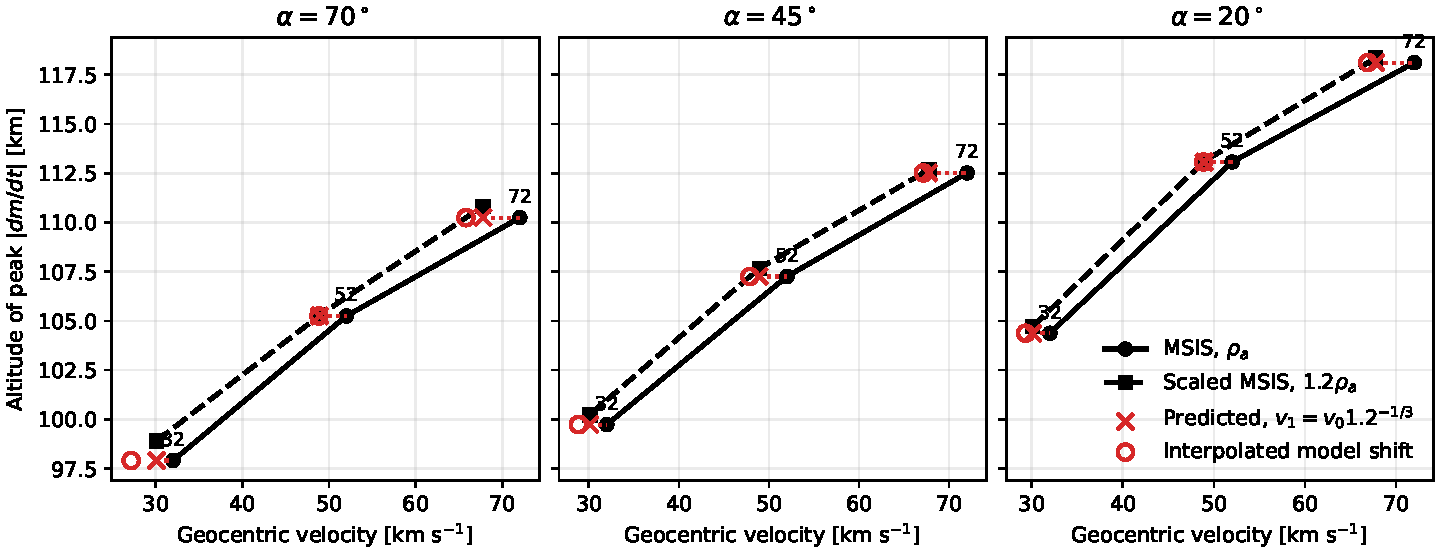
\includegraphics[width=\linewidth]{reproduction/figures/peak_ablation_height-1.20.pdf}
  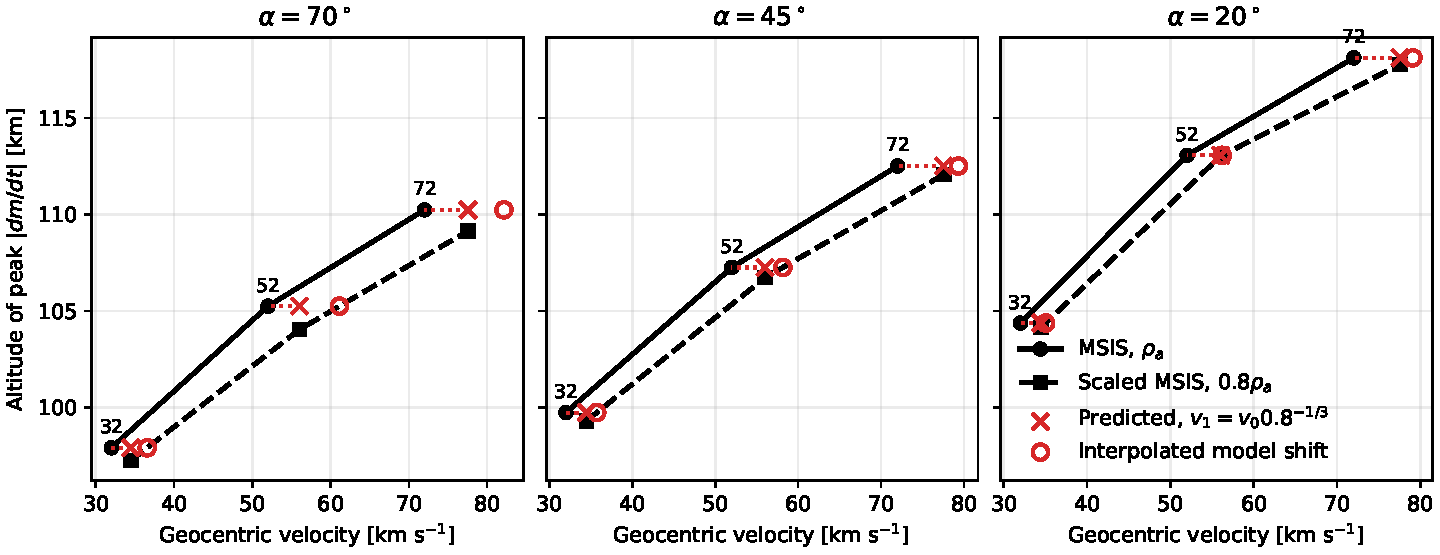
\includegraphics[width=\linewidth]{reproduction/figures/peak_ablation_height-0.80.pdf}
  \caption{Reproduced peak mass-loss altitudes for density factors
  $\gamma=1.2$ (top) and $\gamma=0.8$ (bottom), with the three entry elevation
  angles shown in columns. Baseline entry speeds are 32, 52, and
  72~km~s$^{-1}$. Open red circles show the model velocities obtained by
  piecewise linear interpolation, with endpoint extrapolation as in the
  paper; crosses show the simple $v_1=v_0\gamma^{-1/3}$ prediction.
  Mean inferred density factors are 1.309 and 0.717. Individual printed
  table entries are not all reproduced exactly. Peak heights use
  $|\mathrm{gradient}(m,t)|$ on the adaptive integration samples.
  \scriptprovenance{reproduce_paper.py; paper/make_cabmod_figures.py;
  ablate/src/metablate/models/kero_szasz_2008.py}}
\end{figure}

\begin{figure}[htbp]
  \centering
  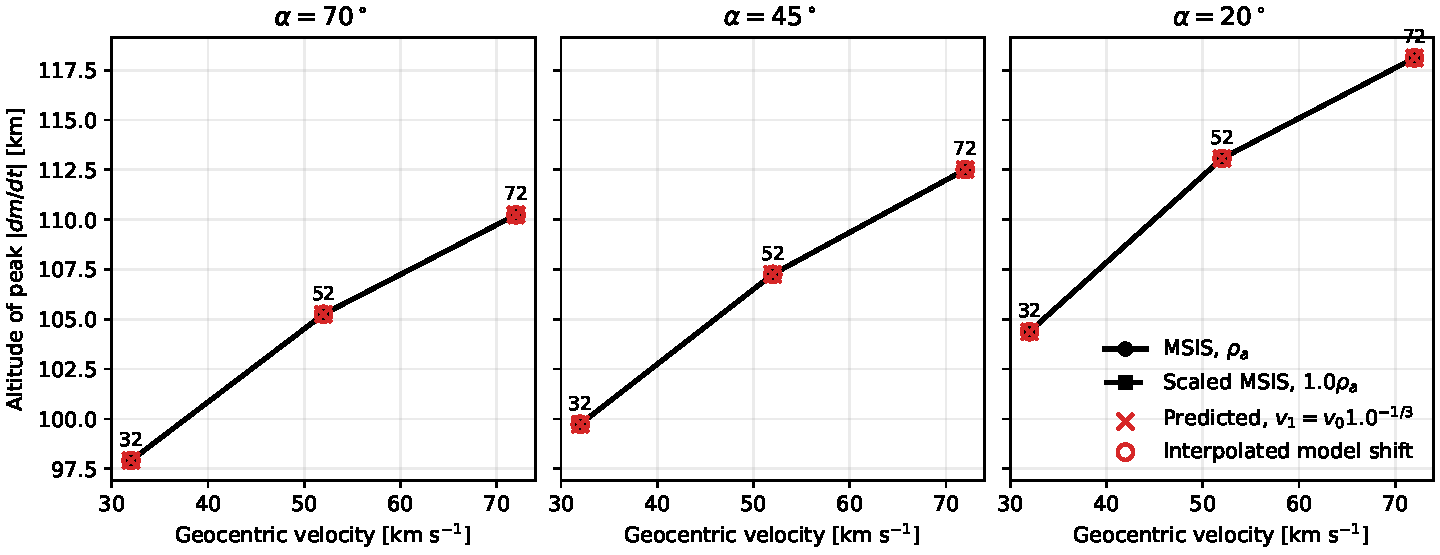
\includegraphics[width=\linewidth]{reproduction/figures/peak_ablation_height-1.00.pdf}
  \caption{Unscaled-atmosphere control, $\gamma=1.0$. Model and simple
  velocity shifts vanish for all three entry elevation angles.
  \scriptprovenance{reproduce_paper.py; paper/make_cabmod_figures.py;
  ablate/src/metablate/models/kero_szasz_2008.py}}
\end{figure}
